\newpage

\section{Luồng xử lý dữ liệu}
\subsection{Chiến lược đồng bộ dữ liệu và cơ chế ghi vào cơ sở dữ liệu}
\label{sec:sync-strategy}
% ============================================================

\subsubsection{Tổng quan}

Sau khi dữ liệu được lấy về từ API nguồn, hệ thống cần quyết định \textit{cách thức ghi} vào cơ sở dữ liệu đích thông qua Prisma ORM. Thay vì áp dụng một phương thức duy nhất cho mọi bảng, hệ thống thiết kế ba chiến lược riêng biệt, mỗi chiến lược phù hợp với đặc thù của từng loại dữ liệu:

\begin{itemize}
  \item \textbf{\texttt{upsert}} — chiến lược mặc định, phù hợp với các bảng nghiệp vụ lớn, dữ liệu có sự thay đổi thường xuyên.
  \item \textbf{\texttt{incremental}} — chiến lược đồng bộ tăng tiến, giúp giảm tải băng thông mạng và cơ sở dữ liệu bằng cách chỉ yêu cầu và ghi nhận những bản ghi có sự thay đổi kể từ lần đồng bộ gần nhất.
  \item \textbf{\texttt{overwrite}} — chiến lược ghi đè toàn bộ, phù hợp với các bảng danh mục nhỏ, cần đảm bảo hệ thống đích hoàn toàn đồng nhất 100\% với hệ thống nguồn.
\end{itemize}

Chiến lược được cấu hình tĩnh trong \textit{Schema Registry} (MongoDB) tại trường \texttt{syncStrategy}, và được áp dụng tự động tại hàm \texttt{syncOneTable()} trong mã nguồn. Thứ tự ưu tiên khi chọn chiến lược diễn ra như sau:

\[
  \texttt{schema.syncStrategy}
  \;\xrightarrow{\text{nếu không có}}\;
  \texttt{upsert} \quad \text{(mặc định)}
\]

Mọi thay đổi về chiến lược đều được áp dụng ngay ở lần đồng bộ tiếp theo mà không cần khởi động lại dịch vụ, nhờ vào cơ chế truy vấn Schema Registry tại thời gian thực thi.

% ------------------------------------------------------------
\subsubsection{Quy trình chung: Phân trang và tải dữ liệu}
\label{sec:sync-pagination}
% ------------------------------------------------------------

Bất kể áp dụng chiến lược nào, hệ thống đều thực hiện \textbf{cơ chế phân trang} khi gọi API nguồn, với kích thước mỗi trang cố định là 5.000 bản ghi (\texttt{BATCH\_LIMIT = 5000}). URL truy vấn được tạo động theo biểu mẫu:

\begin{verbatim}
{baseUrl}{dataFromApi}?page={currentPage}&limit=5000
    [&accessToken={token}]
    [&updatedAfter={lastSyncTime}]   ← chỉ áp dụng khi incremental
\end{verbatim}

Hệ thống tiến hành đọc giá trị \texttt{metadata.totalPages} từ phản hồi của trang đầu tiên để xác định tổng số trang cần duyệt, sau đó lặp cho đến khi tải hết toàn bộ. Mỗi lần tải đều được bao bọc trong cơ chế \textbf{thử lại (retry)} với tối đa 3 lần thao tác nhằm đối phó với lỗi đường truyền mạng.

Hình  mô tả luồng xử lý tổng quát của một bảng dữ liệu, từ thời điểm bắt đầu cho đến khi cập nhật trường \texttt{lastSyncTime}.

\newpage

\begin{figure}[H]
    \centering
    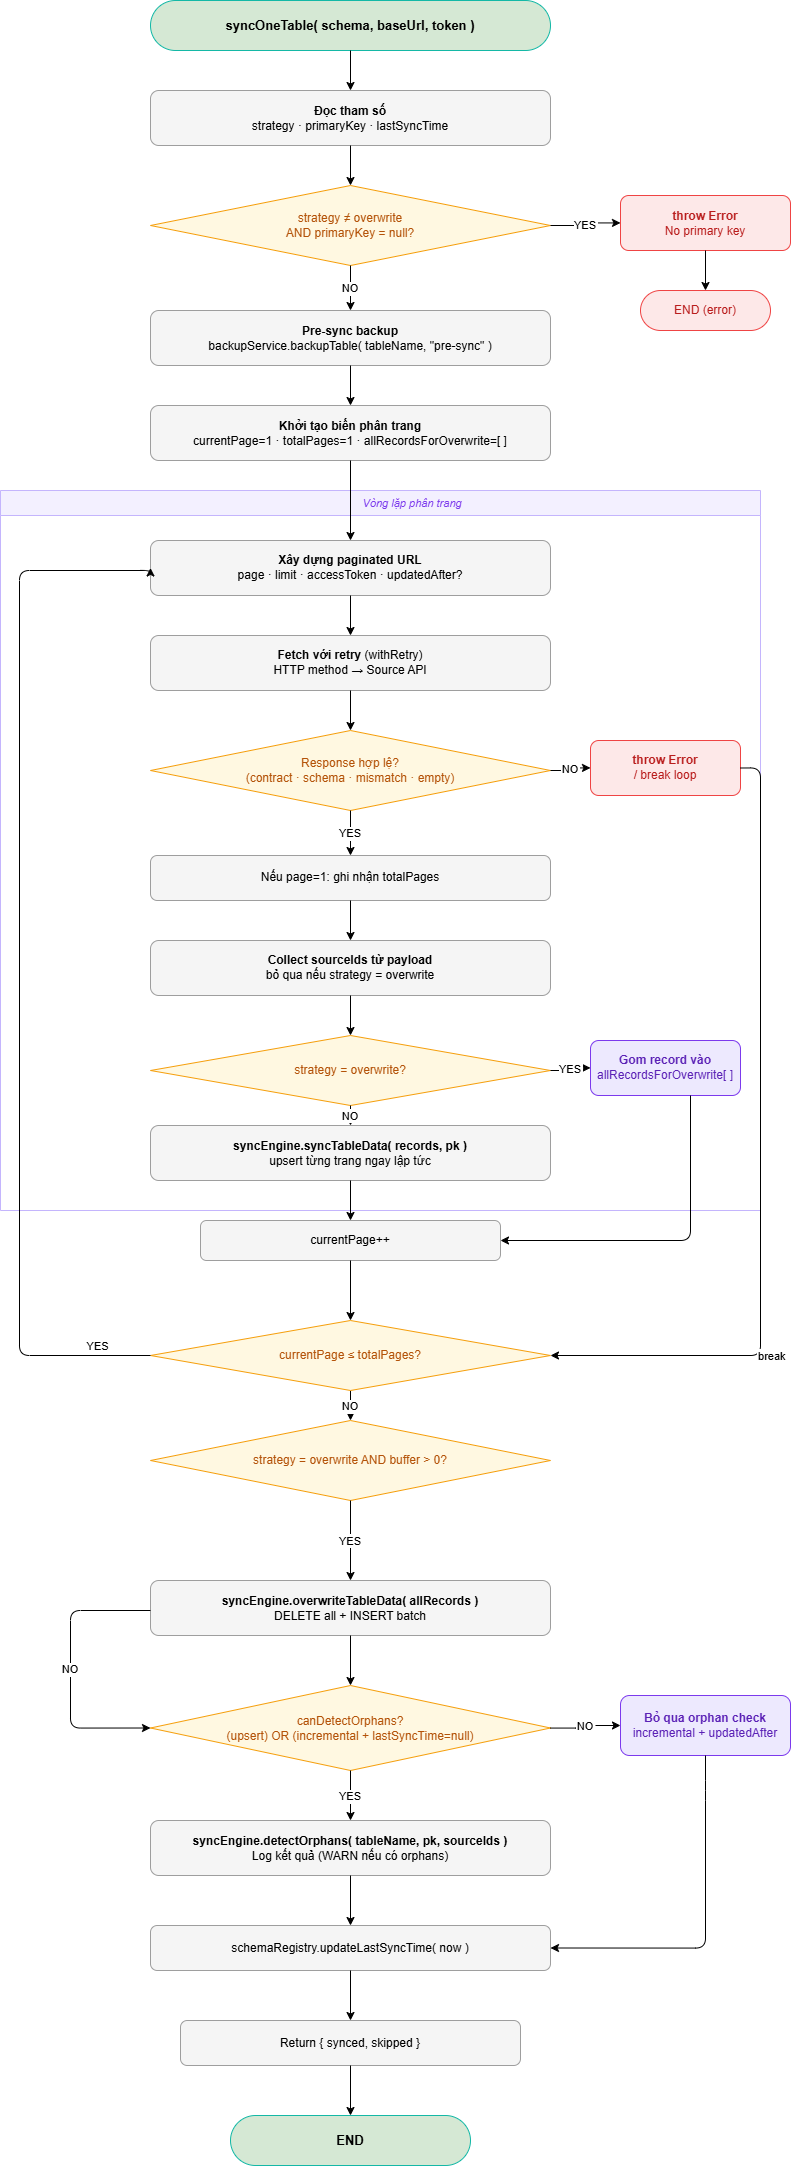
\includegraphics[width=0.5\linewidth]{graphics/SyncOne.png}
    \caption{Cách thức hoạt động của hàm syncOneTable}
    \label{fig:syncone}
\end{figure}


\newpage



% \begin{figure}[H]
% \centering
% \begin{tikzpicture}[
%   node distance=1.4cm,
%   box/.style={rectangle, draw, rounded corners, minimum width=6.2cm,
%               minimum height=0.8cm, text centered, font=\small},
%   decision/.style={diamond, draw, aspect=2.4, text centered,
%                    font=\small, inner sep=1pt},
%   arr/.style={->, >=stealth, thick},
% ]

% \node[box, fill=blue!15] (start)   {Bắt đầu \texttt{syncOneTable()}};
% \node[box, below of=start]  (backup)   {Sao lưu bản ghi hiện tại (MinIO)};
% \node[box, below of=backup]  (strategy) {Đọc \texttt{syncStrategy} + \texttt{lastSyncTime}};
% \node[box, below of=strategy] (fetch)    {Tải trang (retry) — URL kèm \texttt{updatedAfter} nếu incremental};
% \node[box, below of=fetch]    (guard)    {Lọc API Guard + Ràng buộc cấu trúc schema};
% \node[decision, below of=guard, yshift=-0.3cm] (dec) {Chiến lược?};

% \node[box, below left of=dec,  xshift=-3.6cm, yshift=-0.9cm,
%       fill=green!12]  (upsert) {\texttt{upsert}: Cập nhật/chèn toàn bộ};
% \node[box, below of=dec,       yshift=-0.9cm,
%       fill=yellow!20] (incr)   {\texttt{incremental}: Upsert bản ghi trả về};
% \node[box, below right of=dec, xshift=3.6cm,  yshift=-0.9cm,
%       fill=orange!20] (ow)     {\texttt{overwrite}: Đưa vào bộ nhớ đệm RAM};

% \node[decision, below of=incr, yshift=-1.1cm] (morepage) {Còn trang?};

% \node[box, below of=morepage, yshift=-0.4cm,
%       fill=orange!15] (owwrite) {\texttt{overwrite}: DELETE all → INSERT all (transaction)};
% \node[box, below of=owwrite]   (orphan)  {Phát hiện bản ghi mồ côi (upsert / incremental)};
% \node[box, below of=orphan]    (lastsync){Cập nhật \texttt{lastSyncTime} → Schema Registry};
% \node[box, below of=lastsync, fill=blue!15] (done) {Kết thúc};

% \draw[arr] (start)    -- (backup);
% \draw[arr] (backup)   -- (strategy);
% \draw[arr] (strategy) -- (fetch);
% \draw[arr] (fetch)    -- (guard);
% \draw[arr] (guard)    -- (dec);

% \draw[arr] (dec) -- node[above, font=\tiny]{upsert}       (upsert);
% \draw[arr] (dec) -- node[right, font=\tiny]{incremental}  (incr);
% \draw[arr] (dec) -- node[above, font=\tiny]{overwrite}    (ow);

% \draw[arr] (upsert) |- (morepage);
% \draw[arr] (incr)   -- (morepage);
% \draw[arr] (ow)     |- (morepage);

% \draw[arr] (morepage) -- node[right, font=\tiny]{Không} (owwrite);
% \draw[arr] (morepage.west) -- ++(-1.2,0)
%            node[above, font=\tiny]{Có} |- (fetch.west);

% \draw[arr] (owwrite)  -- (orphan);
% \draw[arr] (orphan)   -- (lastsync);
% \draw[arr] (lastsync) -- (done);

% \end{tikzpicture}
% \caption{Luồng xử lý tổng quát của hàm \texttt{syncOneTable()}}
% \label{fig:sync-flow}
% \end{figure}

% ------------------------------------------------------------
\subsubsection{Chiến lược \texttt{upsert} — Mặc định}
\label{sec:strategy-upsert}
% ------------------------------------------------------------

\paragraph{Nguyên lý hoạt động}

Đây là chiến lược \textbf{an toàn và mang tính tổng quát} cao nhất. Với mỗi trang dữ liệu nhận được, hệ thống sẽ tiến hành \texttt{upsert} toàn bộ các bản ghi vào PostgreSQL thông qua Prisma:

\begin{itemize}
  \item Nếu bản ghi chứa \texttt{primaryKey} đã tồn tại $\rightarrow$ thực hiện lệnh \textbf{UPDATE} cho các trường còn lại.
  \item Nếu bản ghi chưa tồn tại $\rightarrow$ thực hiện lệnh \textbf{INSERT} bản ghi mới.
\end{itemize}

Thao tác này đảm bảo tính \textbf{bất biến (idempotent)}: hệ thống có thể chạy lại nhiều lần với cùng một tập dữ liệu đầu vào mà vẫn cho ra cùng một kết quả cuối cùng, không gây ra hiện tượng trùng lặp hay mất mát dữ liệu.

\paragraph{Chi tiết luồng ghi cơ sở dữ liệu}

Trước khi gọi lệnh \texttt{upsert}, mỗi lô bản ghi bắt buộc phải vượt qua bốn lớp tiền xử lý:

\begin{enumerate}
  \item \textbf{Lọc trường dữ liệu (DB Safety Net)} — Loại bỏ các trường không nằm trong định nghĩa lược đồ Prisma. Điều này giúp ngăn chặn lỗi do hệ thống nguồn tự ý bổ sung cột mới mà chưa được thực thi migration trên PostgreSQL.
  \item \textbf{Loại bỏ trùng lặp (Deduplication)} — Nếu dữ liệu nguồn trả về nhiều bản ghi có cùng khóa chính trong cùng một trang, hệ thống chỉ giữ lại bản ghi \textit{xuất hiện sau cùng}. Các bản ghi có khóa chính bị \texttt{null} không bị loại bỏ ở bước này, mà sẽ được giữ lại để đẩy vào nhật ký lỗi (Dead Letter Log).
  \item \textbf{Chuẩn hóa kiểu dữ liệu (Type Normalization)} — Chuyển đổi định dạng từ chuẩn JSON về đúng kiểu dữ liệu khai báo trong Prisma:
        \begin{itemize}
          \item \texttt{DateTime}: chuỗi ISO 8601 $\rightarrow$ Đối tượng \texttt{Date}.
          \item \texttt{Int} / \texttt{Float}: chuỗi chữ số $\rightarrow$ Kiểu số thực.
          \item \texttt{Boolean}: \texttt{"true"} / \texttt{"1"} $\rightarrow$ \texttt{true}.
        \end{itemize}
  \item \textbf{Upsert bất biến và lưu nhật ký lỗi} — Thực hiện lệnh \texttt{prisma[model].upsert()} trong vòng lặp. Nếu một bản ghi bị lỗi (vi phạm ràng buộc dữ liệu duy nhất, sai kiểu...), thông báo lỗi được ghi chú vào \textit{Dead Letter Log} trong MongoDB thay vì bắt buộc dừng toàn bộ tiến trình.
\end{enumerate}

Sau khi hoàn tất, kết quả tổng quan sẽ được ghi vào nhật ký sự kiện MongoDB với các chỉ số báo cáo chi tiết: tổng số bản ghi cần đồng bộ, số lượng bản ghi bị loại bỏ trùng lặp, số bản ghi thành công/thất bại, và mảng chi tiết chứa nguyên nhân lỗi của từng bản ghi.

% ------------------------------------------------------------
\subsubsection{Chiến lược \texttt{incremental} — Bộ lọc tại phía máy chủ}
\label{sec:strategy-incremental}
% ------------------------------------------------------------

\paragraph{Nguyên lý hoạt động}

Chiến lược \texttt{incremental} tận dụng khả năng \textbf{lọc dữ liệu từ phía API nguồn} thông qua việc đính kèm tham số \texttt{updatedAfter}, yêu cầu nguồn chỉ truyền trả những bản ghi đã có sự thay đổi kể từ lần đồng bộ cuối cùng. Cách tiếp cận này giúp tối ưu hóa hiệu năng trên cả hai khía cạnh:

\begin{itemize}
  \item \textbf{Băng thông mạng}: Hệ thống nguồn chỉ trả về một tập con các bản ghi thay vì toàn bộ dữ liệu bảng.
  \item \textbf{Tải cơ sở dữ liệu}: Hệ thống đích chỉ cần thực hiện \texttt{upsert} đúng số lượng bản ghi thực sự mới hoặc bị thay đổi.
\end{itemize}

Mốc thời gian dùng để tạo bộ lọc là trường \texttt{lastSyncTime} trong tài liệu cấu hình (Schema Registry), được hệ thống cập nhật tự động sau mỗi lần đồng bộ thành công.

\paragraph{Quản lý tham số \texttt{updatedAfter}}

Tham số \texttt{updatedAfter} được gắn trực tiếp vào URL truy vấn khi và chỉ khi chiến lược được đặt là \texttt{incremental} \textit{và} bảng đã được đồng bộ ít nhất một lần trước đó (\texttt{lastSyncTime} khác \texttt{null}).

\begin{lstlisting}[caption={Thêm \texttt{updatedAfter} vào URL phân trang},
  label={lst:updateafter-url}]
const updatedAfterParam =
  strategy === 'incremental' && lastSyncTime
    ? `&updatedAfter=${encodeURIComponent(lastSyncTime.toISOString())}`
    : '';
\end{lstlisting}

API nguồn sau khi tiếp nhận tham số này sẽ tiến hành lọc và chỉ trả về các bản ghi thỏa mãn điều kiện \texttt{updatedAt > lastSyncTime}. Toàn bộ số lượng bản ghi trả về sẽ được hệ thống tiến hành \texttt{upsert} thẳng vào cơ sở dữ liệu mà không cần phải thực hiện bước kiểm tra điều kiện thêm một lần nữa.

\paragraph{Trường hợp đồng bộ lần đầu tiên}

Khi \texttt{lastSyncTime = null} (tức bảng chưa từng được đồng bộ), tham số \texttt{updatedAfter} \textbf{sẽ không được thêm} vào URL truy vấn. Khi đó, API nguồn sẽ trả về toàn bộ dữ liệu hiện có — hành vi này tương đương với phương thức \texttt{upsert} (tải toàn phần). Đây là một cơ chế \textbf{khởi tạo ban đầu (bootstrapping)} tự động, giúp quản trị viên không cần phải thiết lập cấu hình thủ công cho lần chạy đầu tiên.

\paragraph{So sánh hiệu năng chiến lược Incremental}

\begin{table}[H]
\centering
\caption{Hiệu quả Incremental: Lọc tại đích (BE-side) và lọc tại nguồn (Server-side)}
\label{tab:incremental-comparison}
\begin{tabular}{lcc}
\toprule
\textbf{Tiêu chí} & \textbf{Lọc tại hệ thống đích} & \textbf{Lọc tại hệ thống nguồn (Mới)} \\
\midrule
Dữ liệu qua mạng  & Toàn bộ bảng (100\%)      & Chỉ tải bản ghi có thay đổi \\
Số trang cần tải  & \texttt{totalPages} đầy đủ & Giảm tỷ lệ thuận theo thay đổi \\
Xử lý tại backend & Lọc \texttt{updatedAt} cho từng dòng & Upsert thẳng vào DB \\
Lượt ghi vào DB   & Chỉ ghi bản ghi thay đổi      & Chỉ ghi bản ghi thay đổi \\
Lợi thế cốt lõi   & Giảm thao tác ghi DB       & Giảm cả thao tác ghi DB và băng thông mạng \\
\bottomrule
\end{tabular}
\end{table}

% ------------------------------------------------------------
\subsubsection{Chiến lược \texttt{overwrite} — Xóa và ghi đè toàn bộ}
\label{sec:strategy-overwrite}
% ------------------------------------------------------------

\paragraph{Nguyên lý hoạt động}

Chiến lược \texttt{overwrite} được thiết kế đặc thù cho các \textbf{bảng danh mục (dimension tables)} với kích thước nhỏ, nơi có yêu cầu cốt lõi là: hệ thống đích phải \textit{hoàn toàn giống hệt} hệ thống nguồn sau mỗi lần chạy. Thay vì cập nhật riêng lẻ từng dòng, hệ thống thực hiện các bước sau:

\begin{enumerate}
  \item \textbf{Tải toàn bộ} dữ liệu từ nguồn, \textbf{lưu đệm toàn bộ vào bộ nhớ RAM} — hệ thống tuyệt đối không thực hiện bất kỳ thao tác ghi cơ sở dữ liệu nào trong giai đoạn phân trang.
  \item \textbf{Sau khi tải xong tất cả các trang}, hệ thống mở một giao dịch duy nhất (\textbf{transaction}) để thực hiện:
        \begin{enumerate}
          \item \texttt{deleteMany(\{\})} — xóa trống toàn bộ dữ liệu bảng hiện tại.
          \item \texttt{createMany(...)} — chèn lại toàn bộ bản ghi mới được tải về.
        \end{enumerate}
\end{enumerate}

Toàn bộ quá trình xóa và chèn được bao bọc trong khối \texttt{prisma.\$transaction()}, đảm bảo \textbf{tính nguyên tử (atomicity)}: nếu quá trình chèn dữ liệu thất bại, thao tác xóa bảng trước đó sẽ lập tức được hoàn tác, ngăn ngừa việc bảng dữ liệu rơi vào trạng thái trống rỗng nửa vời.

\paragraph{Lý do lưu đệm toàn bộ dữ liệu trước khi ghi}

Nếu hệ thống thực hiện thao tác "xóa rồi chèn" tuần tự theo từng trang, bảng dữ liệu đích sẽ bị xóa sạch ngay sau trang đầu tiên và chỉ chứa một lượng nhỏ dữ liệu của trang đó trong khi chờ tải trang tiếp theo. Điều này gây ra \textbf{khoảng thời gian gián đoạn (window downtime)}, ảnh hưởng nghiêm trọng đến các truy vấn đọc đang diễn ra đồng thời của các hệ thống khác. Việc lưu đệm toàn bộ dữ liệu vào RAM rồi mới ghi đè trong một giao dịch duy nhất giúp rút ngắn thời gian gián đoạn xuống mức tối thiểu (chỉ bằng với thời gian thực thi của giao dịch cơ sở dữ liệu).

\paragraph{Miễn trừ cơ chế phát hiện bản ghi mồ côi}

Vì bản chất của \texttt{overwrite} là thực hiện \texttt{DELETE all} trước khi chèn mới, mọi bản ghi bị xóa ở hệ thống nguồn hiển nhiên cũng sẽ bị xóa ở hệ thống đích. Do đó, hệ thống được lập trình để \textbf{bỏ qua hoàn toàn} bước kiểm tra bản ghi mồ côi cho những bảng sử dụng chiến lược này.

\newpage
\subsection{Cơ Chế Retry Trong ETL Pipeline}

\subsubsection{Đặt Vấn Đề}

Trong quá trình đồng bộ dữ liệu từ hệ thống nguồn \textit{myBK} qua REST API,
pipeline ETL phải đối mặt với hai nhóm lỗi có bản chất hoàn toàn khác nhau:

\begin{itemize}
    \item \textbf{Lỗi tạm thời (Transient Errors):} Phát sinh do điều kiện môi
    trường — mạng không ổn định, server nguồn quá tải nhất thời, timeout do
    latency cao. Những lỗi này \emph{có thể tự khỏi} sau một khoảng thời gian
    ngắn.

    \item \textbf{Lỗi nghiệp vụ (Business Errors):} Phát sinh do vi phạm hợp
    đồng dữ liệu — payload sai định dạng, trang phân trang không khớp, khóa
    chính bị thiếu. Những lỗi này \emph{không thay đổi} dù retry bao nhiêu lần,
    vì nguyên nhân gốc rễ nằm ở phía dữ liệu, không phải môi trường.
\end{itemize}

Một cơ chế retry áp dụng đồng nhất cho cả hai nhóm sẽ gây ra hai hệ quả tiêu
cực: lãng phí tài nguyên khi retry lỗi nghiệp vụ không thể phục hồi, và che
khuất các lỗi thực sự cần được xử lý bởi con người.

\subsubsection{Thiết Kế Retry Có Chủ Ý}

Hệ thống áp dụng nguyên tắc \textit{Selective Retry}: chỉ retry các lỗi tạm
thời ở tầng giao tiếp mạng, và để lỗi nghiệp vụ thất bại ngay lập tức
(\textit{fail-fast}) để pipeline có thể ghi nhận và xử lý đúng cách.

\paragraph{Phân Loại Lỗi và Quyết Định Retry}

Bảng~\ref{tab:retry-policy} tổng hợp chính sách retry theo từng tình huống
lỗi trong pipeline.

\begin{table}[H]
\centering
\caption{Chính sách retry theo loại lỗi}
\label{tab:retry-policy}
\renewcommand{\arraystretch}{1.4}
\begin{tabular}{|p{5cm}|c|p{7cm}|}
\hline
\textbf{Tình huống} & \textbf{Retry} & \textbf{Lý do} \\
\hline
Network timeout / \texttt{ECONNREFUSED} &  Có
    & Lỗi tạm thời do môi trường mạng. Server nguồn có thể đã phục hồi sau
      vài giây. \\
\hline
API trả về \texttt{5xx} (server nguồn lỗi) &  Có
    & Server nguồn có thể đang khởi động lại hoặc quá tải nhất thời. Retry
      sau 10 giây có khả năng thành công. \\
\hline
\texttt{[API CONTRACT VIOLATION]} &  Không
    & Payload sai cấu trúc (\texttt{success != true}, thiếu \texttt{payload[]}).
      Retry sẽ nhận lại cùng response sai — không có ý nghĩa. \\
\hline
\texttt{[SCHEMA CONTRACT VIOLATION]} &  Không
    & Payload chứa field chưa định nghĩa trong metadata. Đây là lỗi
      cấu hình cần admin xử lý thủ công. \\
\hline
\texttt{[PAGE MISMATCH]} &  Không
    & Server nguồn trả về sai số trang phân trang. Retry vẫn nhận trang
      sai — cần điều tra phía nguồn. \\
\hline
DB constraint violation (upsert) &  Không
    & Record vi phạm ràng buộc cơ sở dữ liệu sẽ tiếp tục thất bại trong
      mọi lần retry. Chuyển sang \textit{Dead Letter Log} để xử lý riêng. \\
\hline
\end{tabular}
\end{table}

\paragraph{Tham Số Retry}

Pipeline được cấu hình với các tham số sau:

\begin{itemize}
    \item \textbf{Số lần retry tối đa:} 3 lần (tổng cộng 4 lần thử bao gồm
    lần đầu tiên).
    \item \textbf{Khoảng chờ giữa các lần retry:} 10 giây (fixed delay).
    \item \textbf{Phạm vi áp dụng:} Chỉ tầng HTTP fetch — không áp dụng cho
    tầng ghi cơ sở dữ liệu.
\end{itemize}

\paragraph{Cài Đặt}

Retry được đóng gói trong phương thức \texttt{withRetry<T>()} — một generic
wrapper nhận vào một hàm bất đồng bộ và tên ngữ cảnh để ghi log. Phương thức
này được gọi quanh mỗi HTTP request trong vòng lặp phân trang.



Lỗi nghiệp vụ được ném ra \emph{bên ngoài} \texttt{withRetry()} — cụ thể là
sau khi response đã được nhận thành công từ mạng — do đó chúng không bị bắt
bởi vòng lặp retry

\

\subsubsection{Luồng Xử Lý Khi Retry}

Hình~\ref{fig:retry-flow} mô tả luồng quyết định khi một HTTP request thất bại.

\begin{figure}[H]
\centering
\begin{tikzpicture}[
  node distance=1.6cm,
  box/.style={rectangle, draw, minimum width=3.8cm,
              minimum height=0.9cm, text centered, align=center,font=\small},
  decision/.style={diamond, draw, aspect=2.2, text centered,
                   font=\small, inner sep=1pt},
  arrow/.style={->, >=stealth, thick}
]

\node[box] (fetch) {HTTP Request};
\node[decision, below of=fetch, yshift=-0.4cm] (success) {Thành công?};
\node[decision, right of=success, xshift=4.8cm] (retry) {attempt $<$ MAX?};
\node[box, below of=retry, yshift=-0.4cm] (wait) {Chờ 10 giây};
\node[box, right of=retry, xshift=4.2cm] (exceed) {Quá lần thử};
\node[box, below of=success, yshift=-0.4cm] (validate) {Validate nghiệp vụ};
\node[decision, below of=validate, yshift=-0.4cm] (valid) {Hợp lệ?};
\node[box, right of=valid, xshift=3.8cm] (bizfail) {Fail-fast\\(không retry)};
\node[box, below of=valid, yshift=-0.4cm] (sync) {Tiến hành sync};

\draw[arrow] (fetch) -- (success);
\draw[arrow] (success) -- node[above, font=\small]{Không} (retry);
\draw[arrow] (retry) -- node[right, font=\small]{Còn lần} (wait);
\draw[arrow] (wait.west) -- ++(-0.6,0) |- (fetch.east);
\draw[arrow] (retry) -- node[above, font=\small]{Hết lần} (exceed);
\draw[arrow] (success) -- node[right, font=\small]{Có} (validate);
\draw[arrow] (validate) -- (valid);
\draw[arrow] (valid) -- node[above, font=\small]{Không} (bizfail);
\draw[arrow] (valid) -- node[right, font=\small]{Có} (sync);

\end{tikzpicture}
\caption{Luồng quyết định retry trong pipeline ETL}
\label{fig:retry-flow}
\end{figure}

\subsubsection{Đánh Giá}

Thiết kế retry có chủ ý mang lại các lợi ích sau:

\begin{enumerate}
    \item \textbf{Tăng độ bền:} Pipeline tự phục hồi khi gặp lỗi
    mạng tạm thời mà không cần can thiệp thủ công, đặc biệt quan trọng trong
    môi trường ngrok với độ ổn định không cao.

    \item \textbf{Phát hiện lỗi nhanh (Fail-Fast):} Lỗi nghiệp vụ được báo cáo
    ngay lập tức thay vì bị che khuất bởi nhiều lần retry vô ích, giúp rút ngắn
    thời gian phát hiện sự cố từ phía nguồn.

    \item \textbf{Tiết kiệm tài nguyên:} Không lãng phí 30 giây chờ (3 lần
    $\times$ 10 giây) cho các lỗi xác định không thể phục hồi.

    \item \textbf{Log có ngữ cảnh:} Mỗi lần retry được ghi kèm số thứ tự, tên
    bảng, số trang và thông báo lỗi gốc, giúp vận hành dễ dàng truy vết nguyên
    nhân.
\end{enumerate}

\textbf{Hạn chế:} Cơ chế hiện tại sử dụng \textit{fixed delay} (10 giây cố
định). Trong môi trường production với tải cao, chiến lược
\textit{exponential backoff with jitter} sẽ hiệu quả hơn vì tránh được hiện
tượng nhiều client retry đồng thời. Đây là
hướng cải tiến cho phiên bản tiếp theo.

\newpage

\subsection{Phát hiện bản ghi mồ côi (Orphan Detection)}

\subsubsection{Đặt vấn đề}

Các chiến lược đồng bộ \texttt{upsert} và đồng bộ tăng tiến (\texttt{incremental}) chỉ xử lý hai chiều biến động của dữ liệu: thêm mới và cập nhật. Chiều thứ ba - xóa bản ghi tại hệ thống nguồn - hoàn toàn nằm ngoài phạm vi xử lý của hai chiến lược này.

Khi một bản ghi bị xóa tại hệ thống nguồn, nó không còn xuất hiện trong phản hồi của API. Tuy nhiên, bản ghi tương ứng tại hệ thống đích (PostgreSQL) vẫn tồn tại nguyên vẹn vì không có lệnh \texttt{DELETE} nào được phát ra. Theo thời gian, những bản ghi còn lại này tích lũy ngày càng nhiều, tạo ra sự phân mảnh lớn so với dữ liệu nguồn thực tế.

%\begin{figure}[H]
%\centering
%\begin{tikzpicture}[
%  box/.style={rectangle, draw, rounded corners, minimum width=4cm,
%              minimum height=0.8cm, text centered, font=\small},
%  arrow/.style={->, >=stealth, thick}
%]
%\node[box, fill=green!15] (src) {Hệ thống nguồn\\$\{1, 2, 3, 4, 5\}$};
%\node[box, fill=red!15, right of=src, xshift=5cm] (dst)
%    {Hệ thống đích\\$\{1, 2, 3, 4, 5,\ \mathbf{99999}\}$};
%\node[box, fill=orange!20, below of=dst, yshift=-0.8cm]
%    (orphan) {Bản ghi mồ côi: $\{99999\}$};

%\draw[arrow] (src) -- node[above, font=\small]{} (dst);
%\draw[arrow, dashed, red] (dst) -- node[right, font=\small]{chỉ tồn tại ở đây} (orphan);
%\end{tikzpicture}
%\caption{Bản ghi mồ côi: tồn tại ở hệ thống đích nhưng không có ở nguồn}
%\label{fig:orphan-concept}
%\end{figure}
%\end{comment}

Định nghĩa chính thức: một \textbf{bản ghi mồ côi} (orphan record) là bản ghi tồn tại trong cơ sở dữ liệu đích nhưng không xuất hiện trong bất kỳ trang dữ liệu nào được trả về từ API nguồn sau một chu kỳ đồng bộ toàn phần.

\subsubsection{Giải pháp: Phép trừ tập hợp khóa chính}

Trong số các phương án xử lý bản ghi mồ côi, hệ thống lựa chọn phương pháp \textbf{Phép trừ tập hợp khóa chính (ID Set Difference)} — phương án phù hợp nhất với ràng buộc của dự án (API nguồn không hỗ trợ luồng sự kiện thay đổi hay sự kiện xóa).

Ý tưởng cốt lõi:

\begin{equation}
    \text{Orphan IDs} = \text{Destination IDs} \setminus \text{Source IDs}
\end{equation}

Tức là: lấy tập hợp tất cả khóa chính đang tồn tại ở hệ thống đích, trừ đi tập hợp khóa chính thu thập được từ toàn bộ các trang API nguồn. Phần còn lại chính là danh sách các bản ghi không còn tồn tại ở nguồn.

\subsubsection{Quy trình triển khai}

Việc phát hiện bản ghi mồ côi được tích hợp trực tiếp vào cuối hàm \texttt{syncOneTable()} - sau khi vòng lặp phân trang hoàn thành và toàn bộ khóa chính từ nguồn (\texttt{source IDs}) đã được thu thập:

\begin{enumerate}
    \item \textbf{Thu thập khóa chính từ nguồn:} Trong mỗi vòng lặp phân trang, mọi giá trị khóa chính từ \texttt{payload} được thêm vào một tập hợp \texttt{sourceIds}. Bước này không tốn thêm tài nguyên mạng vì dữ liệu đã được tải sẵn.
    \item \textbf{Truy vấn khóa chính tại đích:} Sau khi tải xong tất cả các trang, hệ thống thực hiện một truy vấn \texttt{SELECT} chỉ lấy cột khóa chính từ bảng đích - tránh việc tải toàn bộ bản ghi lên bộ nhớ.
    \item \textbf{Tính toán hiệu tập hợp:} So sánh hai tập hợp, hệ thống trả về danh sách khóa chính chỉ tồn tại ở hệ thống đích.
    \item \textbf{Cảnh báo:} Nếu phát hiện bản ghi mồ côi, hệ thống ghi nhật ký mức độ cảnh báo (\texttt{WARN}) với danh sách mã định danh đầy đủ (hiển thị tối đa 20 mã đầu tiên nếu danh sách quá dài).
\end{enumerate}

\subsubsection{Thiết kế không tự động xóa}

Một quyết định thiết kế quan trọng là hệ thống \textbf{chỉ cảnh báo, không tự động xóa} khi phát hiện bản ghi mồ côi. Quyết định này xuất phát từ ba rủi ro thực tiễn:

\begin{enumerate}
    \item \textbf{Bản ghi mồ côi giả tạo do lỗi API:} Nếu máy chủ nguồn trả về thiếu trang do lỗi phân trang hoặc quá thời gian chờ (timeout), các bản ghi thuộc trang bị thiếu sẽ không có trong \texttt{sourceIds} và bị nhận diện nhầm là bản ghi mồ côi. Việc tự động xóa trong trường hợp này đồng nghĩa với làm mất dữ liệu hợp lệ.
    \item \textbf{Dữ liệu được tạo thủ công:} Một số bảng có thể chứa bản ghi được nhập tay bởi quản trị viên phục vụ mục đích vận hành nội bộ. Những bản ghi này không tồn tại ở nguồn nhưng hoàn toàn hợp lệ tại đích.
    \item \textbf{Tính không thể phục hồi:} Không giống như thao tác chèn hoặc cập nhật, thao tác \texttt{DELETE} không thể hoàn tác (rollback) dễ dàng nếu không có cơ chế sao lưu đầy đủ.
\end{enumerate}

\begin{figure}[H]
\centering
\begin{tikzpicture}[
  node distance=1.5cm,
  box/.style={
      rectangle,
      draw,
      minimum width=4.5cm,
      minimum height=0.9cm,
      text centered,
      align=center,
      font=\small
  },
  decision/.style={
      diamond,
      draw,
      aspect=2.5,
      text centered,
      align=center,
      font=\small,
      inner sep=1pt
  },
  arrow/.style={->, >=stealth, thick}
]

\node[box] (detect)
    {Phát hiện Orphan IDs};

\node[box, below of=detect] (warn)
    {Ghi log WARN + EventLog\\(không tự xóa)};

\node[box, below of=warn, yshift=-0.3cm] (scan)
    {\texttt{POST /integration/scan-orphans}\\(Admin xem lại danh sách)};

\node[decision, below of=scan, yshift=-0.5cm] (confirm)
    {Xác nhận xóa?};

\node[box, below of=confirm, yshift=-0.5cm] (purge)
    {\texttt{POST /integration/purge-orphans}\\(Xóa theo IDs đã chọn)};

\node[box, right of=confirm, xshift=4cm] (skip)
    {Giữ nguyên\\(không làm gì)};

\draw[arrow] (detect) -- (warn);
\draw[arrow] (warn) -- (scan);
\draw[arrow] (scan) -- (confirm);

\draw[arrow] (confirm) -- node[right, font=\small]{Có} (purge);
\draw[arrow] (confirm) -- node[above, font=\small]{Không} (skip);

\end{tikzpicture}

\caption{Quy trình hai bước: phát hiện và xác nhận xóa bản ghi mồ côi}
\label{fig:orphan-flow}
\end{figure}

\subsubsection{API quản lý bản ghi mồ côi}

Hệ thống cung cấp hai điểm cuối (endpoint) riêng biệt để quản trị viên thực hiện quy trình xác nhận hai bước:

\paragraph{Bước 1 — Quét bản ghi mồ côi (Scan)}

\begin{lstlisting}[language=bash, caption={API quét bản ghi mồ côi — chỉ đọc}]
POST /api/v1/integration/scan-orphans
Content-Type: application/json

{ "tables": ["nguoi_hoc"] }
\end{lstlisting}

Điểm cuối này tải toàn bộ dữ liệu từ API nguồn, thực hiện phép trừ tập hợp, và trả về danh sách khóa chính cụ thể. Không có thao tác ghi hoặc xóa nào được thực hiện lên cơ sở dữ liệu.

\begin{lstlisting}[caption={Cấu trúc phản hồi mẫu từ API scan-orphans}]
[{
  "tableName": "nguoi_hoc",
  "primaryKey": "id",
  "orphanCount": 1,
  "orphanIds": [99999]
}]
\end{lstlisting}

\paragraph{Bước 2 — Xóa có xác nhận (Purge)}

\begin{lstlisting}[language=bash, caption={API xóa bản ghi mồ côi — yêu cầu truyền ID tường minh}]
POST /api/v1/integration/purge-orphans
Content-Type: application/json

{
  "tableName": "nguoi_hoc",
  "primaryKey": "id",
  "ids": [99999]
}
\end{lstlisting}

Quản trị viên bắt buộc phải sao chép danh sách \texttt{orphanIds} từ kết quả của bước 1 và truyền lại một cách tường minh vào yêu cầu này. Cơ chế này đảm bảo không thể xảy ra việc vô tình xóa hàng loạt do lỗi lập trình hay gọi API không có chủ đích.

Mỗi lần xóa được ghi nhận vào nhật ký sự kiện với đầy đủ thông tin: tên bảng, khóa chính, số lượng ID được yêu cầu xóa, và số lượng bản ghi thực tế đã bị xóa.

\subsubsection{Giới hạn của phương pháp}

Phương pháp trừ tập hợp khóa chính có hiệu quả cao trong điều kiện hiện tại của dự án, song cần lưu ý một giới hạn quan trọng: orphan detection tự động trong sync chỉ chạy khi fetch toàn bộ (upsert hoặc incremental lần đầu), muốn kiểm tra orphan trên incremental cần gọi POST /integration/scan-orphans riêng — endpoint đó luôn fetch toàn bộ source.
Với cấu trúc dữ liệu hiện tại (ví dụ: bảng \texttt{nguoi\_hoc} chứa hơn 68.000 bản ghi), thời gian quét mất khoảng 3 phút — đây là mức chi phí chấp nhận được cho một tác vụ vận hành định kỳ, nhưng không phù hợp nếu yêu cầu kiểm tra theo thời gian thực. Hướng cải tiến lâu dài là yêu cầu hệ thống nguồn cung cấp điểm cuối API \texttt{/changes?since=<timestamp>} để chỉ trả về danh sách các khóa chính bị xóa trong một khoảng thời gian cụ thể.

\subsection{Thông Báo Qua Email Sau Khi Pipeline Chạy Xong}
\label{sec:notification}

\subsubsection{Đặt vấn đề}

Sau khi một pipeline đồng bộ dữ liệu hoàn thành --- dù thành công hay thất
bại --- hệ thống cần chủ động thông báo đến quản trị viên mà không yêu cầu
họ phải theo dõi log liên tục. Cơ chế thông báo qua email giải quyết nhu
cầu này: kết quả của mỗi lần chạy pipeline được gửi tự động đến địa chỉ
email cấu hình sẵn ngay khi job kết thúc.

\subsubsection{Công nghệ sử dụng}

Hệ thống sử dụng thư viện \textbf{Nodemailer} tích hợp trong \texttt{NotificationService}
(NestJS) để gửi email qua giao thức \textbf{SMTP}. Mặc định kết nối tới
Gmail (\texttt{smtp.gmail.com:587}) với xác thực TLS, nhưng có thể đổi sang
bất kỳ SMTP server nào qua biến môi trường.

Kết nối SMTP được khởi tạo một lần khi module load. Nếu biến môi trường
\texttt{SMTP\_USER} hoặc \texttt{SMTP\_PASSWORD} chưa được cấu hình, service
tự động tắt tính năng email mà không làm crash ứng dụng --- đảm bảo môi
trường phát triển không bắt buộc phải có SMTP.

\subsubsection{Điểm kích hoạt}

\texttt{NotificationService} được gọi tại cuối cả hai pipeline đồng bộ trong
\texttt{DataIntegrationService}:

\begin{itemize}
  \item \textbf{Full Integration Pipeline} --- đồng bộ toàn bộ các bảng
        có trạng thái \texttt{stable}.
  \item \textbf{Custom Integration Pipeline} --- đồng bộ một tập bảng do
        admin chỉ định.
\end{itemize}

Tùy kết quả, một trong hai phương thức được gọi:

\begin{itemize}
  \item \texttt{sendJobSuccessSummary()} --- khi toàn bộ bảng đồng bộ thành
        công (\texttt{status = done}).
  \item \texttt{sendJobFailureAlert()} --- khi có ít nhất một bảng thất bại
        (\texttt{status = partial\_success} hoặc \texttt{failed}).
\end{itemize}

\subsubsection{Nội dung email}

Mỗi email được render dưới dạng \textbf{HTML} với bố cục bảng, gồm các
trường sau:

\begin{figure}
    \centering
    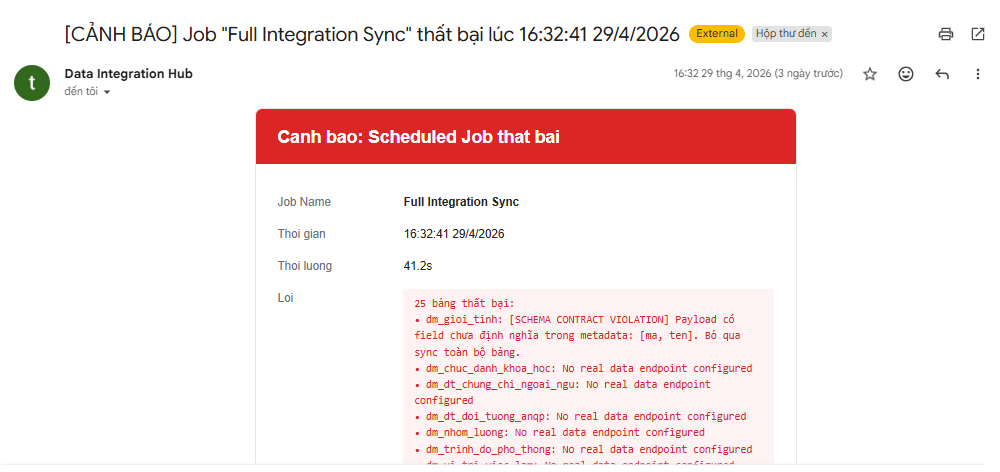
\includegraphics[width=1\linewidth]{graphics/email_aleart.png}
    \caption{Minh họa mail cảnh báo}
    \label{fig:dashboard-ui}
\end{figure}

\subsubsection{Cấu hình biến môi trường}

\begin{table}[H]
\centering
\caption{Biến môi trường cho NotificationService}
\label{tab:notification-env}
\begin{tabular}{lll}
\hline
\textbf{Biến} & \textbf{Mặc định} & \textbf{Mục đích} \\
\hline
\texttt{SMTP\_HOST}     & \texttt{smtp.gmail.com} & SMTP server \\
\texttt{SMTP\_PORT}     & \texttt{587}            & Cổng SMTP (TLS) \\
\texttt{SMTP\_USER}     & ---                     & Địa chỉ email gửi \\
\texttt{SMTP\_PASSWORD} & ---                     & App Password của Gmail \\
\texttt{ALERT\_EMAIL\_TO} & ---                   & Địa chỉ nhận cảnh báo \\
\hline
\end{tabular}
\end{table}

Với Gmail, \texttt{SMTP\_PASSWORD} phải là \textbf{App Password} (16 ký tự)
được tạo tại \textit{Google Account $\to$ Security $\to$ 2-Step Verification
$\to$ App passwords} --- không dùng mật khẩu tài khoản thông thường.

\subsubsection{Luồng xử lý}

\begin{figure}[H]
\centering
\begin{tikzpicture}[
  node distance=1.4cm,
  % Tất cả box dùng chung minimum width/height để đồng đều
  box/.style={
    rectangle, rounded corners=4pt,
    draw=black, fill=white,
    minimum width=3.6cm, minimum height=0.8cm,
    font=\small\bfseries, align=center, text=black,
    line width=0.8pt
  },
  % Diamond giữ aspect ratio hợp lý
  dec/.style={
    diamond, aspect=3.5,
    draw=black,
    font=\small\bfseries, align=center, text=black,
    line width=0.8pt
  },
  % Khối fail/success cùng kích thước với box
  side/.style={
    rectangle, rounded corners=4pt,
    draw=black,
    minimum width=2.8cm, minimum height=0.8cm,
    font=\small\bfseries, align=center, text=black,
    line width=0.8pt, dashed
  },
  arr/.style={
    -{Stealth[length=5pt,width=4pt]},
    thick, black
  },
  lbl/.style={font=\small, fill=white, inner sep=2pt}
]

  \node[box] (pipe)  {Pipeline kết thúc};
  \node[dec,  below=1.0cm of pipe]  (dec)  {status?};
  \node[side, right=2.4cm of dec]   (suc)  {sendJobSuccess\\Summary()};
  \node[side, left=2.4cm of dec]    (fail) {sendJobFailure\\Alert()};
  \node[box,  below=1.0cm of dec]   (smtp) {Nodemailer\\SMTP};
  \node[box,  below=1.0cm of smtp]  (mail) {Email đến\\ALERT\_EMAIL\_TO};

  \draw[arr] (pipe) -- (dec);
  \draw[arr] (dec.east) -- node[lbl, above]{done}   (suc.west);
  \draw[arr] (dec.west) -- node[lbl, above]{failed} (fail.east);
  \draw[arr] (suc.south)  -- ++(0,-0.5) -| (smtp.east);
  \draw[arr] (fail.south) -- ++(0,-0.5) -| (smtp.west);
  \draw[arr] (smtp) -- (mail);

\end{tikzpicture}
\caption{Luồng gửi email thông báo sau khi pipeline kết thúc}
\label{fig:notification-flow}
\end{figure}